\section{Problem}
Given $n$ items: $S=[i_1, i_2, \_, i_n]$ and a positive integer $m \leq n$, the goal is to select $m$ items of $S$ \emph{uniformly at random} (each item can be picked with probability $\frac{1}{n}$).

There are two variants:
\begin{itemize}
    \item $n$ known;
    \item $n$ unknown.
\end{itemize}

We will analyze the solution in 2 different computing models:
\begin{itemize}
    \item 2-level memory model;
    \item streaming model: limited memory so you must decide for the element one at a time.
\end{itemize}

We assume \verb|rand(a, b)| to return a random value in the range $[a, b]$ with uniformly distribution.
To pay less I/Os we assume to access chosen elements from left to the right in sorted order for position.

\section{Known n, 2-level memory}
We have $S[1, n]$ with pointers to actual items, since we want to avoid to work on real $S$ we copy it's content on $S'$ and then execute the algorithm:
\begin{verbatim}
    for s in {0, _ , m-1}
        p = rand(1, n-s)
        pick S'[p]
        swap S'[p] with S'[n-s]
\end{verbatim}
Ex:
\begin{figure}[H]
    \centering
    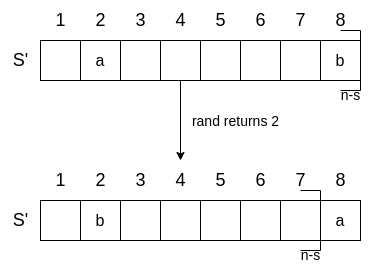
\includegraphics[width=250px]{images/3_Random_Sampling/random_sampling_1.png}
    \caption{random sampling with $n = 8$}
\end{figure}
As we can notice at each step we exclude an element moving it at the end of the array.
At the end of the algorithm the end of the array will contain the selected items.

This algorithm runs in linear time but jumps around in the array.

We would like to get an algorithm which provides only the indexes of the elements so that we can avoid access to disk: 
\begin{verbatim}
    D = {}
    while |D| < m:
        p = rand(1, n)
        if p not in D:
            insert p in D
\end{verbatim}
This algorithm has a huge problem: the more i go ahead, the more probable it is to find an element which is already in D:
$$
    P(p \in D) = \frac{|D|}{n} < \frac{m}{n}
$$
in particular if $m \leq \frac{n}{2} \implies P(p \in D) < \frac{1}{2}$

NB: supposing $m < \frac{n}{2}$ is okay since if we have $m > \frac{n}{2}$ we could reverse the problem choosing the element that we won't take, so the upper bound to consider is always $m = \frac{n}{2}$.

So we have $O(m)$ expected time, and on average 2 runs for each $p$, in terms of I/Os: $min \{ m, \frac{n}{B} \}$.

\section{Known n, streaming model}
I see $i_1, i_2, \_, i_n$ and I want to decide to keep or not for each element when I see it, without the capability to store them.
Let's suppose $m=1$ and we want to choose:
\begin{itemize}
    \item $i_1 \xrightarrow{} \frac{1}{n}$;
    \item $i_2 \xrightarrow{} \frac{1}{n-1}$;
    \item $i_3 \xrightarrow{} \frac{1}{n-2}$;
    \item ...
    \item $i_n \xrightarrow{} \frac{1}{n-n+1}$;
\end{itemize}
There is no possibility of not choosing any element since the last element has probability of $\frac{1}{n-n+1} = 1$.

NB: The predicate \emph{keep an element with probability} $p$ can be evaluated with $rand(0, 1) \leq p$ using the rand function as a function which returns a real number in the range $[0, 1]$.

To prove that the probability are correct let's estimate $\mathbb{P}(\text{picking } i_j)$ given that I've not picked any other items.
Let' prove by induction that every element is chosen with probability $\frac{1}{n}$:
$$
    \mathbb{P}(\text{picking } i_j) = \mathbb{P}(\text{pick } i_j) \cdot \mathbb{P}(\text{not pick }i_1, i_2, \_, i_{j-1}) = \frac{1}{n-j+1}\cdot \left(1 - \frac{j-1}{n} \right)
$$
$$
    = \frac{1}{n-j+1}\cdot \left(\frac{n - j + 1}{n} \right) = \frac{1}{n}
$$

For the generic $m$ we pick $i_j$ with probability:
$$
    \frac{m-s}{n-j+1}
$$
with $s$ the number of already extracted items.

Let's suppose $s=0$ with $m$ items left to see:
$$
    \mathbb{P}(\text{picking } i_{n-m+1}) = \frac{m-s}{n-j+1} = \frac{m}{n-(n-m +1)+1} = \frac{m}{m} = 1
$$
so the last $m$ items will surely be taken.

NB: the formula is the generic case of choosing an element with probability: 
$$
    \frac{\#\text{elements we need to pick}}{\#\text{available elements}}
$$

NB: The main problem with all the approaches we followed is that we extract $n$ random numbers which is too much, we won't cover algorithms that extract just $m$ random numbers but there exists.

Example: $S = {a, b, c, d, e}$, $n = 5$, $m = 1$, $p = {0.5, 1, 0.1, 0.3, 0.7}$
\begin{itemize}
    \item $a: 0.5 \leq \frac{1}{5} = 0.2 \implies$ discard item;
    \item $b: 1 \leq \frac{1}{4} = 0.25 \implies$ discard item;
    \item $c: 0.1 \leq \frac{1}{3} = 0.33 \implies$ keep item.
\end{itemize}
Suppose $m = 2$:
\begin{itemize}
    \item $c: 0.1 \leq \frac{2}{3} \implies$ keep item;
    \item $d: 0.3 \leq \frac{1}{2} \implies$ keep item.
\end{itemize}

\section{Unknown n, streaming model}
\subsection{Reservoir Sampling}
\begin{verbatim}
    R[1,m] = S[1,m] //we pick the first m elements in S
    
    for each next S[j], j >= m+1:
        h = rand(1, j)
        if (h <= m)
            R[h] = S[j]
    return R
\end{verbatim}

We can prove the correctness by induction: the base case with $n = m$ items should produce probability of bringing those items equals to 1 and the first step of the algorithm solves it.
The inductive hypothesis for $n-1$ is that every item $i_j$ for $j = 1, 2, \_, n-1$ is picked with $\mathbb{P} = \frac{m}{n-1}$.
Let's prove that every item $i_j$ for $j=1, 2, \_, n$ has $\mathbb{P} = \frac{m}{n}$:
$$
    \mathbb{P}(i_n \text{ is picked}) = \frac{m}{n}
$$
because I extract \verb|rand(1, j)| with $j=n$ and pick the item if \verb|rand(1, n) <= m| so:
$$
    \mathbb{P}(i_j \text{ is picked, } j < n) = 
$$
$$
    \mathbb{P}(i_j \text{ is in } R \text{ at step } n-1 \land (i_n \text{ is not picked} \lor i_n \text{ is picked but } i_j \text{ is not kicked out})) =
$$
$$
    \mathbb{P}(i_j \in R \text{ at step } n-1) \cdot \left[ \mathbb{P}(i_n \text{ is not picked}) + \mathbb{P}(i_n \text{ is picked} \land i_j \text{is not overwritten}) \right]=
$$
$$
    \frac{m}{n-1} \cdot \left[ \left( 1 - \frac{m}{n} \right) + \left( \frac{m}{n} \right) \cdot \left( \frac{m-1}{m} \right) \right] = \frac{m}{n-1} \cdot \left[ 1 - \frac{m}{n} + \frac{m-1}{n} \right] =
$$
$$
    \frac{m}{n-1} \cdot \left[ 1 - \frac{1}{n} \right] = \frac{m}{n-1} \cdot \left[ \frac{n-1}{n} \right] = \frac{m}{n}
$$

Ex: $S = a, b, c, d, e, f$, $m=2$
\begin{itemize}
    \item $R = [a, b]$, $h = 3$, $c$ not chosen;
    \item $R = [a, b]$, $h = 4$, $d$ not chosen;
    \item $R = [a, b]$, $h = 2$, $e$ chosen instead of $b$;
    \item $R = [a, e]$, $h = 3$, $f$ not chosen.
\end{itemize}

In this algorithm we are generating too many random numbers.

NB: another way of computing: 
$$
    \mathbb{P}(i_n \text{ is not picked}) + \mathbb{P}(i_n \text{ is picked} \land i_j \text{is not overwritten}) = 
$$
is:
$$
    \mathbb{P}(\text{not extracting j}) = 1 - \frac{1}{n}
$$

\subsection{Heap-based approach}
The main concept is: given $S=a, b, c, d, e, f, \_$ for each element we extract a probability in the range $[0, 1]$ and we keep an heap for priority with size $m$, so at the end we return the heap content.

Ex: $H = \{ (b, 0.2), (a, 0.1) \}$
\begin{itemize}
    \item $(c, 0.05)$: discard;
    \item $(d, 0.3)$: insert: $H = \{ (b, 0.2), (c, 0.1) \}$;
    \item $(e, 0.9)$: insert: $H = \{ (e, 0.9), (b, 0.2) \}$;
    \item $(f, 0.2)$: discard.
\end{itemize}
the returned elements are: $d, e$.

% TODO: add the heap-based algorithm

